%% Overleaf			
%% Software Manual and Technical Document Template	
%% 									
%% This provides an example of a software manual created in Overleaf.

\documentclass{ol-softwaremanual}

% Packages used in this example
\usepackage{graphicx}  % for including images
\graphicspath{{./images/}}
\usepackage{microtype} % for typographical enhancements
\usepackage{minted}    % for code listings
\usepackage{amsmath}   % for equations and mathematics
\usepackage{wrapfig}   % for wrapping text around figures
\setminted{style=friendly,fontsize=\small}
\renewcommand{\listoflistingscaption}{List of Code Listings}
\usepackage{hyperref}  % for hyperlinks
\usepackage[a4paper,top=4.2cm,bottom=4.2cm,left=3.5cm,right=3.5cm]{geometry} % for setting page size and margins
\usepackage{listings}
\lstset{language=bash}

% Custom macros used in this example document
\newcommand{\doclink}[2]{\href{#1}{#2}\footnote{\url{#1}}}
\newcommand{\cs}[1]{\texttt{\textbackslash #1}}

\tolerance=1
\emergencystretch=10pt
\hyphenpenalty=10000
\hbadness=10000

% Frontmatter data; appears on title page
\title{Recycling Robot\\Documentation}
\version{1.0.0}
\author{Rimvydas Kersys}
\softwarelogo{
\includegraphics[width=8cm]{images/logo}}

\begin{document}

\maketitle

\tableofcontents
\listoflistings
\newpage

\section{Project Overview}

This project implements an autonomous waste-sorting system using a KUKA KR180-2 industrial robot, a vision-based detection pipeline, and a Raspberry Pi–controlled motorised gripper.

The system is designed to detect recyclable objects on a conveyor belt, classify them using a machine learning model, and command the robot to pick and place each item into the correct bin.

System Workflow:
\begin{enumerate}
    \item A complete sorting cycle operates as follows:
    \item The vision model processes a live camera feed and detects waste objects.
    \item The detected object’s position is transformed into robot coordinates.
    \item The robot moves to the target position.
    \item The Raspberry Pi actuates the gripper to grasp the object.
    \item The robot transports the object to the appropriate disposal bin.
    \item The robot returns to its home position and awaits the next detection.
\end{enumerate}

The system is modular. Vision processing, robot motion, and gripper control operate as independent components communicating over a local network.

\section{System Architecture}

% TODO: Introduce System Architecture section
\newpage
\subsection{Hardware Architecture}

% TODO: Write something about the Hardware Architecture
\begin{figure}[h!]
    \centering
    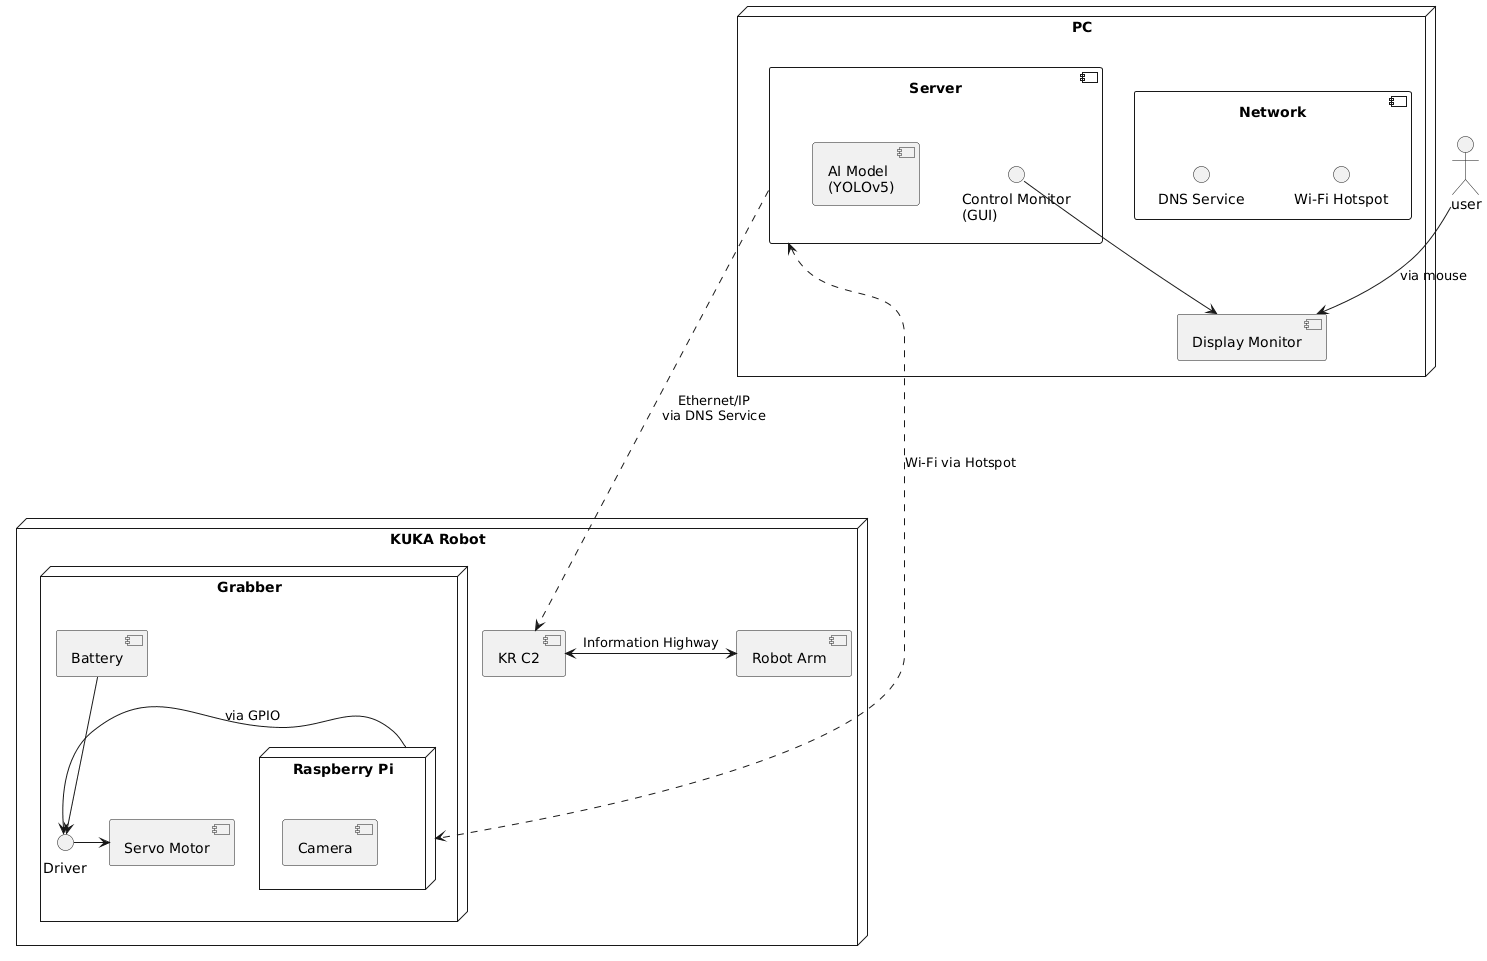
\includegraphics[width=1\linewidth]{images/Component Diagram.png}
    \caption{Full Hardware Component Diagram}
    \label{fig:hardwareArchitecture}
\end{figure}

\newpage
\subsection{Software Architecture}

% TODO: Write something about the Software Architecture

\begin{figure}[h!]
    \centering
    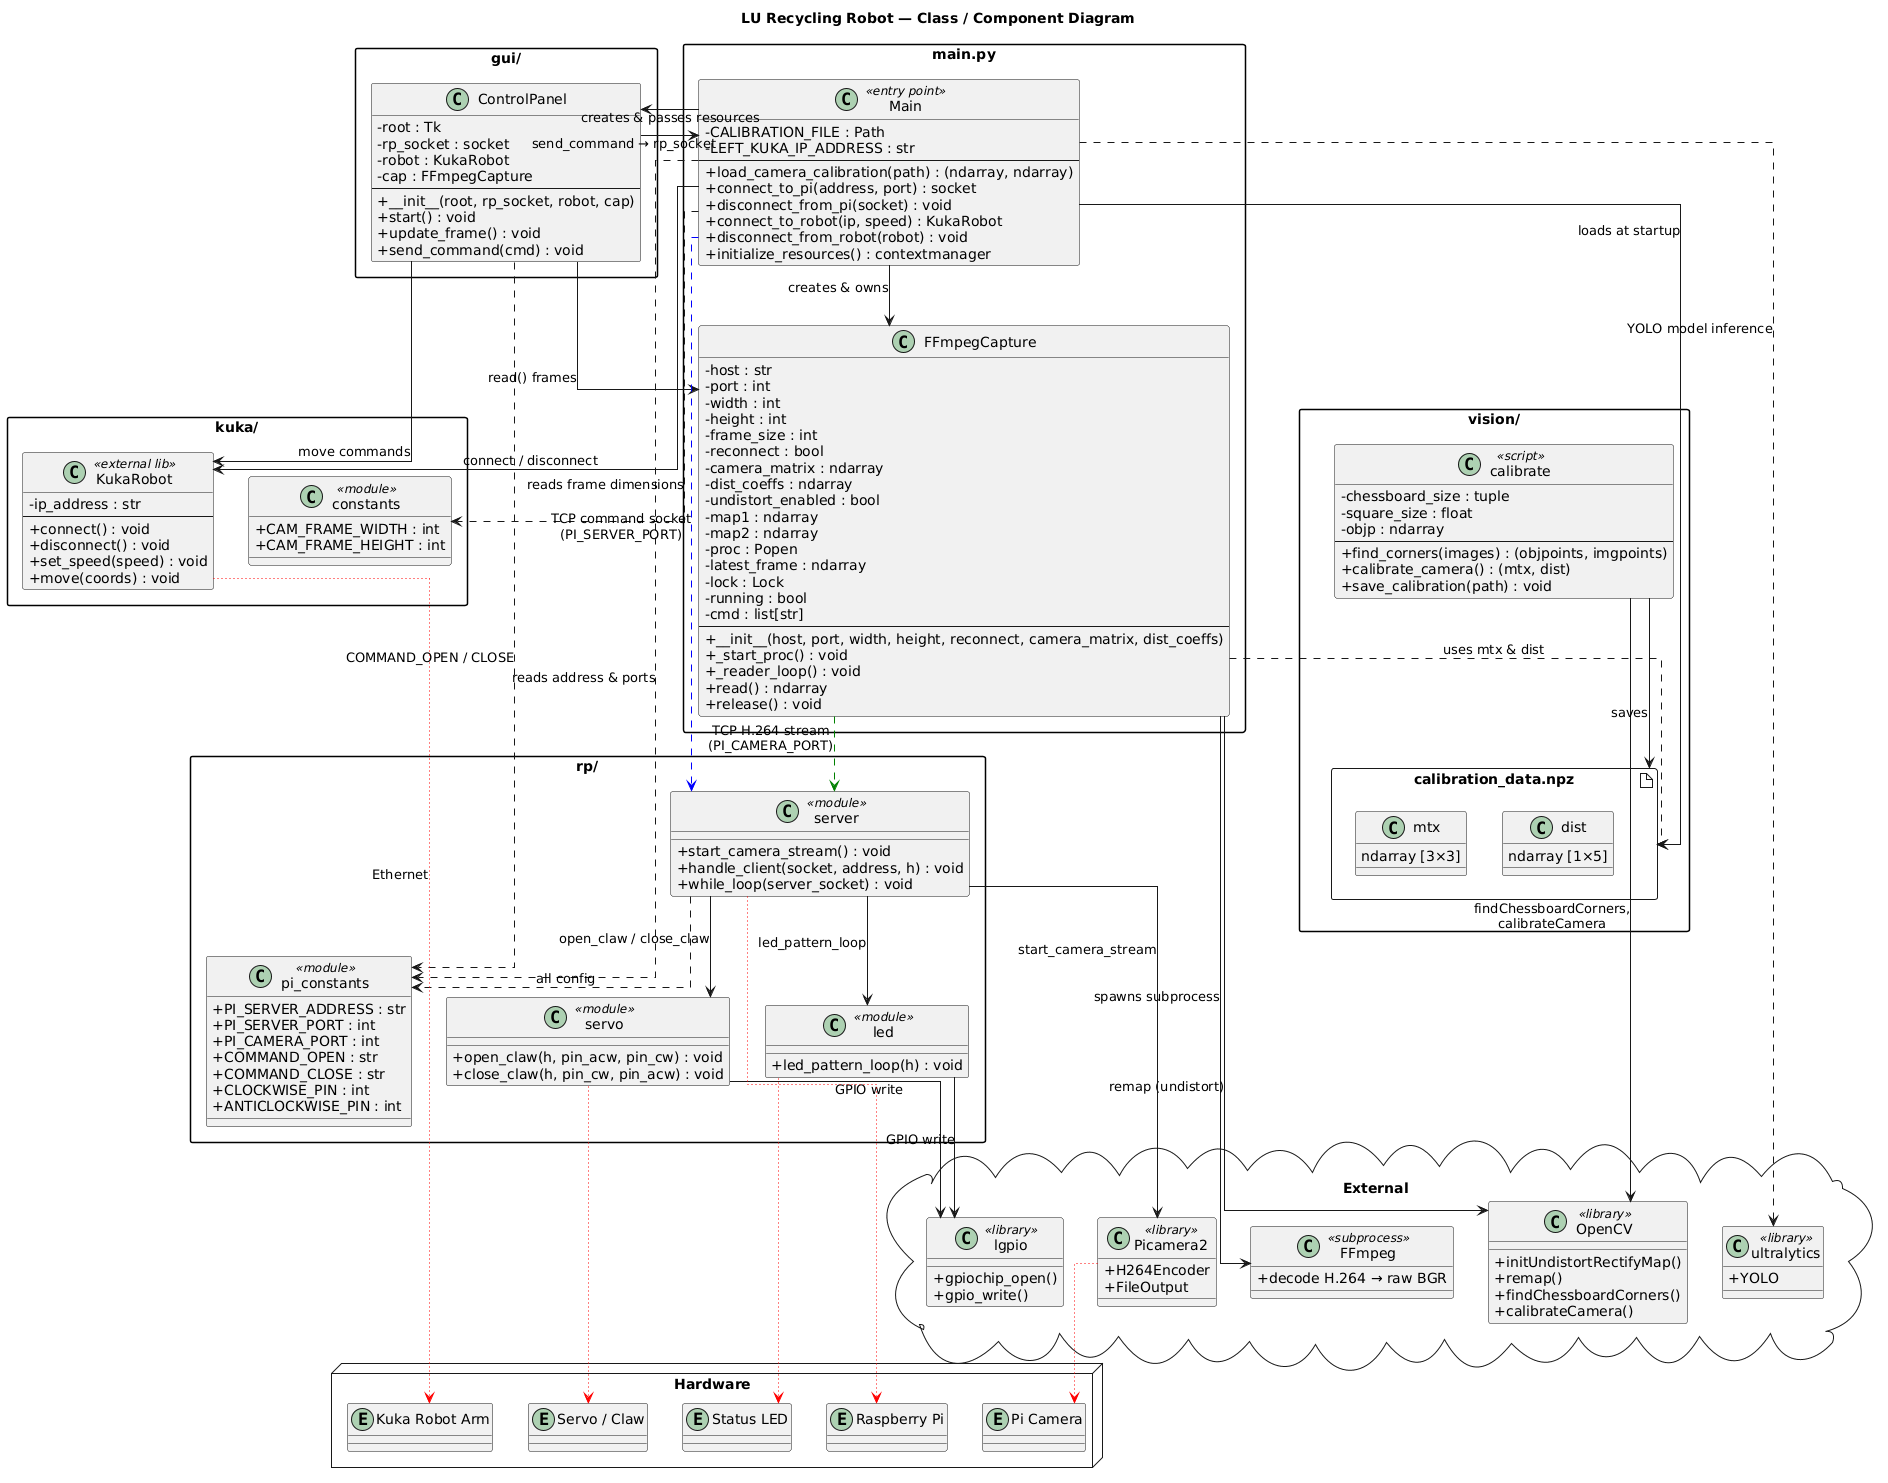
\includegraphics[width=1\linewidth]{images/Software Diagram.png}
    \caption{Full Software Component Diagram}
    \label{fig:softwareArchitecture}
\end{figure}

\section{Hardware Setup}

\subsection{Robot}

The robot position is based on the position of its tool. Depending on the grabber size and angle, you may want to calibrate the robot to these. It is important to note that the robot is not entirely accurate and may still go to a location which is off the intended location by up to 2-3mm or more if these errors are related to the angle of the tool.

The robot can also be calibrated (mastered) to help alleviate some location inconsistencies however this is out of scope for this document.

Currently, the robot's position is not absolute. The robot is visually not angled correctly. Despite this, absolute location errors are accounted for via software.

\subsection{Raspberry Pi}

\begin{wrapfigure}{r}{0.5\textwidth} % If done correctly shoudl appear on the right hand side of the bullet point list above
    \centering
    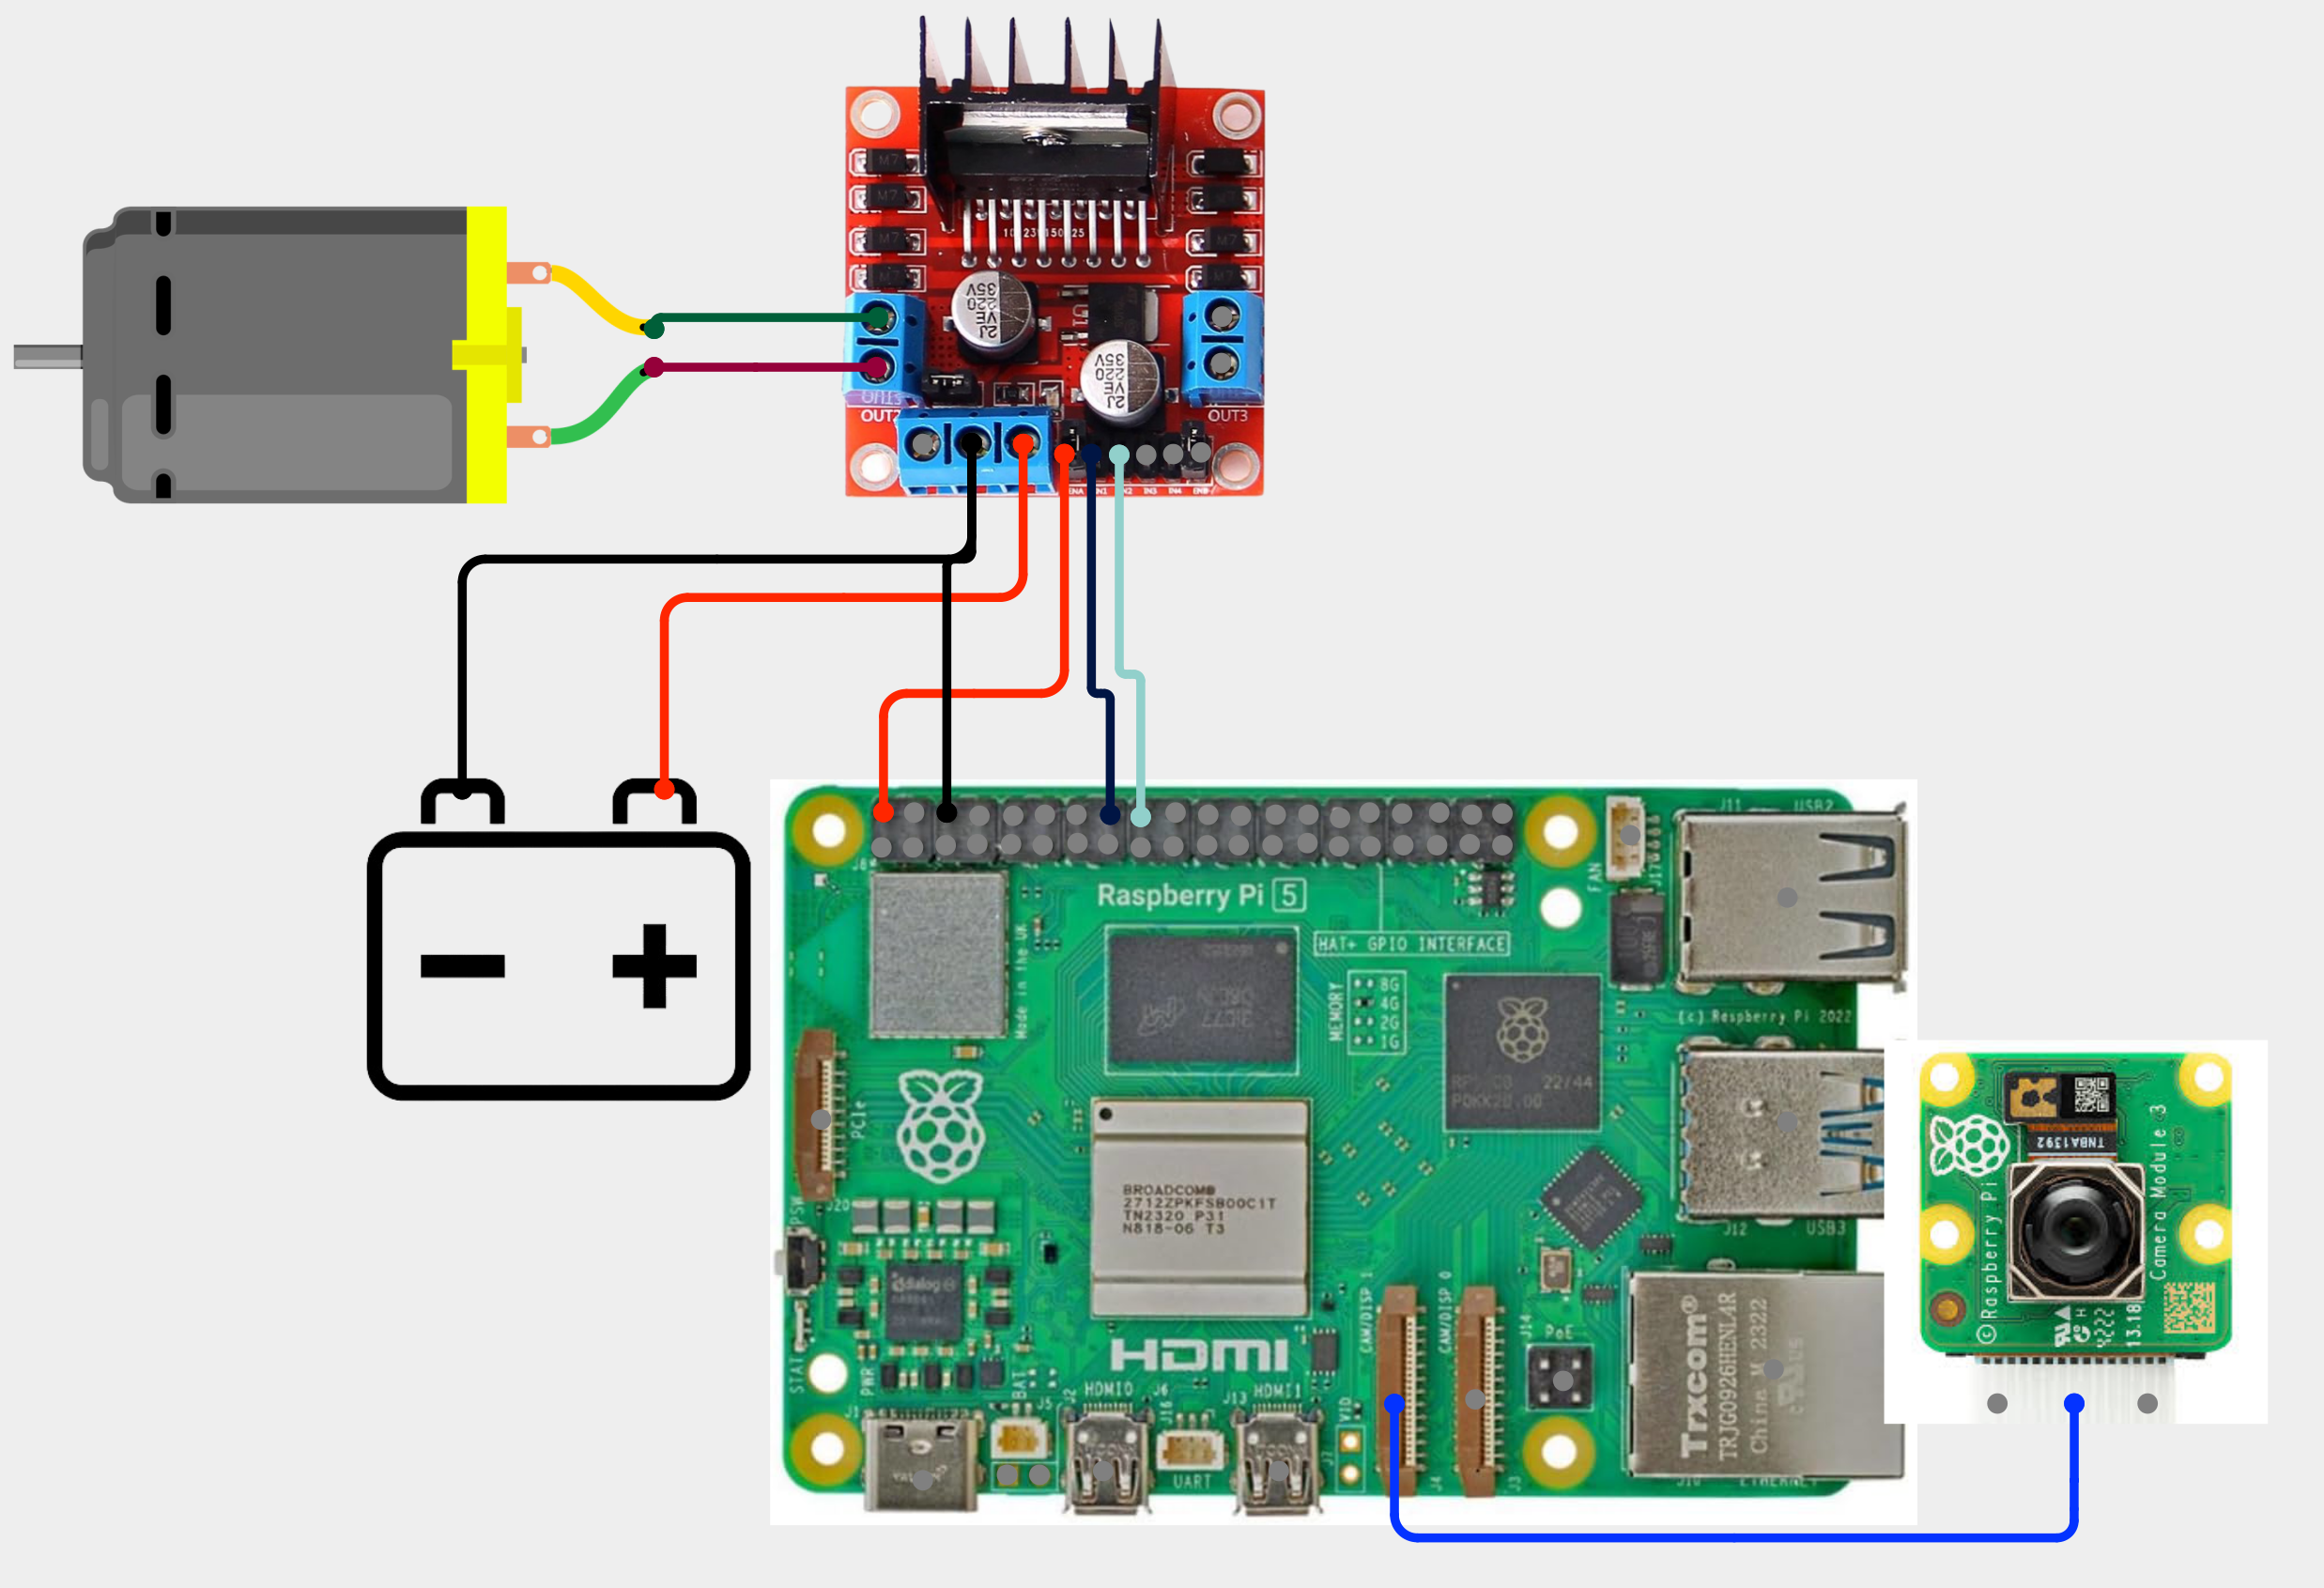
\includegraphics[width=1\linewidth]{images/GPIOWiring.png}
    \caption{Components wired together}
    \label{fig:GPIOWiring}
    \vspace{-70pt}
\end{wrapfigure}

The Raspberry Pi acts as the embedded controller for the:
\begin{itemize}
    \item PiCamera Module 3
    \item L298N motor driver
    \item Gripper motor
\end{itemize}

\subsubsection{Hardware Used}

\begin{itemize}
    \item Raspberry Pi 5
        \footnote{While a Raspberry Pi 5 is used in this setup, lower-power models (like the Raspberry Pi Zero) may be used if performance requirements permit.}
    \item PiCamera Module 3
    \item L298N DC Motor Driver
    \item 12V Battery
    \item Portable Charger (Pi power supply)
    \item 3-6V DC Motor (gripper actuation)
\end{itemize}

\subsubsection{Camera Positioning}

The PiCamera is mounted beneath the robot arm and positioned approximately perpendicular to the conveyor belt. This orientation minimises perspective distortion and simplifies coordinate transformation in software.

If mounted facing downwards, autofocus inconsistencies may occur. Focus correction should be handled in software or manually adjusted if using older camera modules.

\subsubsection{Motor Driver Considerations}

The L298N introduces an approximate 2V voltage drop between supply and motor output.

For this reason:
\begin{itemize}
    \item A 6V battery is insufficient for long-term operation
    \item A 12 V batter is recommended
    \item The resulting motor voltage (~10V after drop) provides:
    \begin{itemize}
        \item Faster actuation (~2s vs ~5s)
        \item Improved torque margin
        \item More reliable gripping under load
    \end{itemize}
\end{itemize}
If variable motor speed control is required, the enable (ENA) pin may be connected to a PWM-capable GPIO pin instead of the fixed 5V pin as in Fig \ref{fig:GPIOWiring}.

\subsection{Gripper \& Motor Driver}

The Motor and Driver are both affixed to the arm such that the motor rotates a bolt perpendicular to the arm. 

\section{Communication \& Networking}

The system operates over a local Wi-Fi network hosted by the server machine

\subsection{Network Architecture}

\begin{itemize}
    \item The server broadcasts a hotspot with:
    \begin{itemize}
        \item SSID: kukaman
        \item Password: kukawifi
    \end{itemize}
    \item The Raspberry Pi connects automatically to this network.
    \item The robot controller communicates with the server over Ethernet
\end{itemize}

\subsection{IP addressing}

The dnsmasq service is used on the server machine to
\begin{itemize}
    \item Assign IP addresses to the two KR C2 controllers
    \item Provide lightweight DHCP functionality
    \item Maintain stable local addressing
\end{itemize}

To verify the service is running, run
\begin{lstlisting}[language=bash, caption="verifying the dnsmasq service"]
    $ journalctl -xefu dnsmasq
\end{lstlisting}
in the server machine's terminal.

\subsection{Communication}
\begin{enumerate}
    \item Vision detection runs on the server
    \item Coordinates of object are calculated
    \item Commands are sent to the robot controller
    \item Gripper commands are sent to the Raspberry Pi
    \item Any relevant status messages are logged for debugging
\end{enumerate}
All communication occurs within the local network and does not require internet access.

\section{System Service}

The Raspberry Pi runs a "\lstinline{systemd}" service called \lstinline{rpi-server.service} to ensure
\begin{itemize}
    \item Automatic startup on boot
    \item Controlled deployment on runtime files
    \item Automatic restart on failure
\end{itemize}

\subsection{Runtime File Protection}
On service start:
\begin{enumerate}
    \item A \lstinline{/local} directory is created
    \item All files from \lstinline{/rp} are copied into \lstinline{/local}
    \item The program runs from \lstinline{/local}
\end{enumerate}

This design prevents:
\begin{itemize}
    \item Runtime corruption during code edits
    \item Partial updates while the system is running
    \item Inconsistent execution states
\end{itemize}

To apply updated code do one of the following:
\begin{lstlisting}[language=bash, caption="Updating Raspberry Pi code]
    $ systemctl restart rpi-server.service
    --------------------------------------
    $ sudo reboot
\end{lstlisting}

The service is configured to automatically recover in the event of a crash.


\section{Robot Motion \& Control}

The robot operates in tool-based coordinate space.

\subsection{Coordinate Mapping}

In software, object positions detected by the vision system are: 
\begin{enumerate}
    \item Extracted in image coordinates
    \item Converted to real-world measurements
    \item Robot coordinates calculated relative to current robot position
\end{enumerate}

\subsection{Motion Sequence}

For each object detected:
\begin{enumerate}
    \item Move to safe, pre-grasp, height
    \item Open gripper
    \item Descend vertically
    \item Close Gripper
    \item Ascend to safe clearance height
    \item Move to correct bin location
    \item Release object by opening gripper
    \item Close gripper
    \item Return to home position
\end{enumerate}

\section{Safety Considerations}

This system uses an industrial robotic arm and moving mechanical components. Proper safety procedures must always be followed.

To do this, it is essential that operators of the robot complete a risk assessment to ensure that all risks are noticed and procedures are put in place in the event that risks occur.

\subsection{Room Specific Safety Measures}
In the room in which the robots are based, it is essential to wear steel capped boots and ensure that all foods and drinks are kept in sealed containers.

\subsection{Robot Safety}
Under no circumstances should the robot be operated whilst another person is inside of the cage with the robot.

When operating in \lstinline{auto} or \lstinline{Ext.} mode, the Robot will emergency stop if the safety gate is open. However, in both \lstinline{T1} and \lstinline{T2} modes, the robot can still be manually controlled even whilst the gate is open. Ensure that nobody is inside the cage and that the gate is closed before operating the robot.

\subsection{Electrical Safety}
Under no circumstances should the KR C2 controller be opened while operating. Take necessary precautions as described in the KR C2 manual before opening the controller.

\subsection{Mechanical Safety}
The gripper creates many pinch points during operation. Before operating the gripper, ensure that all hands are clear of the gripper.

\section{Setup \& Deployment Guide}
\subsection{Raspberry Pi}

\subsubsection{Imaging the Raspberry Pi}
First, create a Raspberry Pi OS image for the respective Pi device. Ensure when making the image to enable SSH and set the correct Wi-Fi name and password. During operation, the Server machine broadcasts a Wi-Fi connection via hotspot with SSID: "kukaman" and password: "kukawifi" which should be used when robot is running. However, any other Wi-Fi connection can be used when first initialising.

\subsubsection{Connecting via SSH}
When using the terminal, there are 2 methods which can be used to connect to the Raspberry Pi.
\begin{lstlisting}[language=bash, caption="How to SSH into a Raspberry Pi"]
$ ssh {deviceName}@{userName}
# The currently used Raspberry Pi would be kuka@KukaPi

$ ssh {deviceName}@{IPAddress} 
# The currently used Raspberry Pi would be kuka@10.42.0.218
\end{lstlisting}

If using an app to access the Raspberry Pi, such as VNC Viewer. You will likely need to provide the IP address.

To find out the IP address of the Raspberry Pi, you may use
\begin{lstlisting}[language=bash, caption="Finding the IP address of a Raspberry Pi via terminal on personal device"]
$ arp -a
\end{lstlisting}
or you may first SSH into it via the terminal using a username and then use
\begin{lstlisting}[language=bash, caption="Finding the IP address of a Raspberry Pi via on device terminal"]
$ hostname -I
\end{lstlisting}
which will output the Raspberry Pi's IP address. Or, you may instead connect an external display to the Raspberry Pi and using an external keyboard and mouse hover over the Wi-Fi icon %TODO: FACT CHECK THIS
to see the Raspberry Pi' IP address

\subsubsection{Deployment}
Finally, to get the Raspberry Pi to run the program on start up:
\begin{lstlisting}[language=bash, caption="Raspberry Pi Deployment"]
    $ git clone https://github.com/Rimichu/LU-Recycling-Robot
    $ cd LU-Recycling-Robot/rp

    $ # Copy (and if it exists, replace) the service
    $ sudo cp -fr rpi-server.service 
        /etc/systemd/system/rpi-server.service

    $ # Start Service (May require password)
    $ systemctl start rpi-server.service

    $ # Check to ensure that the service is working
    $ journalctl -xefu rpi-server.service
\end{lstlisting}

When the service starts, the service will create a new directory "local" and copy all files from the /rp directory there to be used during runtime. This will allow you to change code in the /rp directory with no danger to the program during run time. Upon changing code, to use the new code just run either

\begin{lstlisting}[language=bash, caption="Restarting the Raspberry Pi Service"]
    $ systemctl restart rpi-server.service  # Restarts the service
    $ sudo reboot                           # Restarts the Raspberry pi
\end{lstlisting}

which will again re-copy all files and run the program.

\subsection{Server}

Clone the repository, create and open the kuka environment:
% TODO: github repository will have to be changed in future (ownership will change)
\begin{lstlisting}[language=bash, caption="Server Deployment"]
    $ git clone https://github.com/Rimichu/LU-Recycling-Robot
    $ cd LU-Recycling-Robot
    $ conda env create -f env.yaml
    $ conda activate kuka
\end{lstlisting}

% TODO: There is likely things missing here which are AI related

\subsection{Start-up Instructions}

% TODO: Explain what the HMI is, perhaps a screenshot
% TODO: Provide button by button presses to make self administrator
\begin{enumerate}
    \item Turn on all necessary devices
    \begin{enumerate}
        \item Turn on the Kuka Controller (KR C2) via Lever and follow any on screen instructions until the Human Machine Interface (HMI) panel appears
        \item Ensure KR C2 is set to Auto Mode
        \item Start up the server machine (Password: kuka)
        \item Place and plug in 12V battery into driver
        \item Place portable charger on robot arm ensuring enough clearance for other components
        \item Plug in portable charger into raspberry pi
        \item Turn off overhead lights
    \end{enumerate}
    \item On the server machine, ensure that the dnsmasq service is running correctly via the terminal
    \begin{lstlisting}[language=bash, caption="Checking and Restarting the DNS service on Server machine"]
# Check on the service
$ journalctl -xefu dnsmasq
# Use Ctrl+C to continue using the terminal

# Restart the service
$ systemctl restart dnsmasq
    \end{lstlisting}
    \item On the KR C2 controller, make yourself administrator \footnote{See \hypertarget{Debugging \& Troubleshooting}{Debugging \& Troubleshooting} if the safety gate was opened whilst the KR C2 was turned on}
    \begin{enumerate}
        \item Configure $\rightarrow$ User Group $\rightarrow$ Administrator (Password: kuka)
        \item Ensure Num Lock is Disabled $\rightarrow$ Ctrl+Esc $\rightarrow$ IssacStartC3Bridge
        \item Alt+Tab into the Kuka HMI
    \end{enumerate}
    \item Inside the HMI, run the C3BI\_RUN program
    \begin{enumerate}
        \item Press enter when selected
        \item Reduce program speed to a recommended 50\%
        \item Press the green button once to get robot to its starting position (current position as default)
        \item Press the green button again to begin robot program
    \end{enumerate}
    \item In the Server machine's terminal:
    \begin{lstlisting}[language=bash, caption="Running Server code"]
$ cd LU-Recycling-Robot # Ignore if already in directory
$ conda activate kuka   # Ignore if already in kuka environment
$ python3 main.py
    \end{lstlisting}
\end{enumerate}

\subsection{Power-down Instructions}
\begin{enumerate}
    \item Server Machine
    \begin{enumerate}
        \item Ensure program is off by one of the following in order of safety:
        \begin{enumerate}
            \item Quit Safely Button
            \item Exiting the program via exit button
            \item Using Ctrl+C in the terminal
        \end{enumerate}
        \item Power off server machine
    \end{enumerate}
    \item Kuka Robot
    \begin{enumerate}
        \item Press "Stop" button to stop any actively running program.
        \item TODO: How to navigate to fresh start turn off
        \item Power off Kuka Controller (KR C2) via lever
    \end{enumerate}
    \item Motor Battery
    \begin{enumerate}
        \item Unplug 12V battery
        \item take 12V battery off the mount to charge
    \end{enumerate}
    \item Raspberry Pi
    \begin{enumerate}
        \item Unplug portable charger from Raspberry pi
        \item Take portable charger off the mount to charge
    \end{enumerate}
\end{enumerate}



\section{Debugging \& Troubleshooting}\hypertarget{Debugging \& Troubleshooting}{}

If the gate is opened whilst the KR C2 is operating, the KR C2 will no longer be able to run code. To fix this, ensure the gate is closed and flip the lever off and on to soft reset the KR C2.

\section{Limitations \& Known Issues}

\section{Future Work}

\appendix

% This document is an example of a software manual created using \LaTeX\ and Overleaf. It provides a nice clean format for producing this type of technical document. 
% Simply start writing your document and use the Recompile button to view the updated PDF preview. Examples of commonly used commands and features can be found in the sections below, to help you get started.
% To change the logo shown on the front page, simply upload your own logo image file (via the file-tree menu) to replace the default logo.pdf file. 
% Once you're familiar with the editor, you can find various project settings in the Overleaf menu, accessed via the button in the very top left of the editor. To view tutorials, user guides, and further documentation, please visit our \doclink{https://www.overleaf.com/learn}{help library}. If you haven't used \LaTeX\ before, our \doclink{https://www.overleaf.com/learn/latex/Learn_LaTeX_in_30_minutes}{Learn \LaTeX\ in 30 minutes} tutorial is an excellent place to start.
% For large documents, it can be useful to split the document into multiple source files.
% Double-clicking on text in Overleaf's PDF preview will take you directly to the corresponding code in the editor.
% \section{Including code samples}

% \input{code-samples}

% \section{Some further examples to get started}

% \input{further-examples}

\end{document}
